\section{Problem (4)}
	In the \cref{fig:hwb_problem4}, three particles of mass $m = 3.2 \ kg$ are fastened to three rods of length $d = 0.45 \ m$ and negligible mass. The rigid assembly rotates about point $O$ at angular speeed $\omega = \ 9.0 \ rad/s$. About $O$,

	\begin{figure}[H]
		\begin{center}
			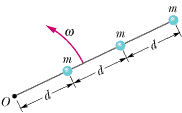
\includegraphics[scale=1]{hwb_problem4}
			\caption{Illustration of Problem 4}
			\label{fig:hwb_problem4}
		\end{center}
	\end{figure}

	\subsection{Question (a)}

		What is the rotational inertia of the assembly?

		\textbf{R:}

		\begin{align}
			m_{1} = \ &m_{2} = m_{3} = m& \notag \\
			r_{1} = \ &d& \notag \\
			r_{2} = \ &2d& \notag \\
			r_{3} = \ &3d& \notag \\
			I = \ & \sum_{i} m_{i} r_{i}^{2}& \notag \\
			= \ & \left(m_{1}r_{1}^{2}\right) + \left(m_{2}r_{2}^{2}\right) + \left(m_{3}r_{3}^{2}\right)& \notag \\
			= \ & m\left[(d)^{2} + (2d)^{2} + (3d)^{2}\right]& \notag \\
			= \ & m\left[14(d)^{2}\right]& \notag \\
			= \ & (14)(3.2 \ kg)(0.45 \ m)^{2}& \notag \\
			= \ & (44.8 \ kg)\left(0.2025 \ m^{2}\right)& \notag \\
			= \ & 9.0720 \ kg \times m^{2}&
		\end{align}

	\subsection{Question (b)}

		What is the magnitude of the angular momentum of the asembly?

		\textbf{R:}

		\begin{align}
			L = \ &I \omega& \notag \\
			= \ &\left(9.0720 \ kg \times m^{2} \right) (9.0 \ rad/s)& \notag \\
			= \ &81.6480 \ kg \times m^{2}/s&
		\end{align}
